\documentclass[usenames,xcolor={dvipsnames, table}]{beamer}
\usepackage[utf8]{inputenc}
\usepackage{lmodern}
\usepackage{verbatim}
\usetheme{uniud}
\usepackage{xparse}
\usepackage[spanish,es-tabla,es-nodecimaldot, es-nosectiondot, es-lcroman, es-noquoting]{babel}
\usepackage{subcaption}
\usepackage{array}
\usepackage{multirow}
\usepackage{multicol}
\usepackage{booktabs}
\usepackage{booktabs}
	\setlength\heavyrulewidth{0.9pt}

\usepackage{threeparttable}
\usepackage{amsmath}
\usepackage{nccmath}
\usepackage{etoolbox}
\usepackage{siunitx}

\makeatletter
\pretocmd\env@cases{\def\@rowc@lors{}}{}{}
\pretocmd\start@align{\def\@rowc@lors{}}{}{}
\makeatother

\newsavebox{\bmatrixbox}
\newenvironment{colorbmatrix}
  {\begin{lrbox}{\bmatrixbox}
   \mathsurround=0pt
   $\displaystyle
   \begin{bmatrix}}
  {\end{bmatrix}$%
   \end{lrbox}%
   \usebox{\bmatrixbox}%
   \kern-\wd\bmatrixbox
   \makebox[0pt][l]{$\left[\vphantom{\usebox{\bmatrixbox}}\right.$}%
   \kern\wd\bmatrixbox
}

% \ExplSyntaxOn
% \NewDocumentCommand{\convertto}{mm}
% % #1 = em or ex (or any other unit)
% % #2 = dimen to convert
% {
% 	\texttt{#2~=~\fp_to_decimal:n { (#2)/(1#1) }#1}
% }
% \ExplSyntaxOff

%%% Some useful commands
% pdf-friendly newline in links
\newcommand{\pdfnewline}{\texorpdfstring{\newline}{ }} 
% Fill the vertical space in a slide (to put text at the bottom)
\newcommand{\framefill}{\vskip0pt plus 1filll}


\title[Universidad Nacional Experimental del Táchira]{Laboratorio virtual de sistemas de control clásicos y difusos utilizando software libre}
\date[Marzo 2020]{Marzo 11, 2020}
\author[Proyecto Especial de Grado]{
  \textbf{Autor}: \hfill \\ Br. Kleiver J. Carrasco M. \\ \vspace{10pt} \textbf{Tutor}: \\ MSc. Ing. Juan R. Vizcaya R.
}

\institute{
	Universidad Nacional Experimental del Táchira

	Vicerrectorado Académico
	
	Decanato de Docencia
	
Departamento de Electrónica
}


\begin{document}

\begin{frame}
	\titlepage
\end{frame}

\begin{frame}
	\frametitle{INTRODUCCIÓN}
	\vspace{20pt}

	\begin{block}{Planteamiento del problema}
		\begin{itemize}
			\large 
			\item ¿Es posible realizar un laboratorio para el análisis de sistemas de control con software libre?
			\item ¿Cumpliría con los requisitos para analizar, diseñar y simular sistemas de control?
			\item ¿Cómo se desempeñaría en comparación con otras herramientas?
		\end{itemize}
	\end{block}

	\begin{block}{¿Por qué ``Laboratorio Virtual''?}
		\begin{figure}
				\centering
				\begin{subfigure}[b]{0.2\linewidth}
					
\includegraphics[width=\linewidth]{imagenes/logoMATLAB}
				\end{subfigure}
				\hspace{0.8cm}
				\begin{subfigure}[b]{0.25\linewidth}
					
\includegraphics[width=\linewidth]{imagenes/logoSciLab}
				\end{subfigure}
				
			\end{figure}
	\end{block}
\end{frame}

\begin{frame}
	\frametitle{OBJETIVOS}
	\vspace{20pt}
	\begin{block}{Objetivo General}
		Desarrollar un laboratorio virtual de sistemas de control clásicos y difusos utilizando software libre.
	\end{block}
	
	\begin{block}{Objetivos específicos}
		\begin{enumerate} 
			\item Estudiar los sistemas de control clásicos.
			\item Estudiar el diseño de controladores difusos tipo Mamdani.
			\item Codificar las rutinas de análisis, diseño y simulación de sistemas de control necesarias.
			\item Realizar la interfaz gráfica de un laboratorio de sistemas de control virtual.
			\item Comparar los resultados obtenidos con dos herramientas de corte similar.
		\end{enumerate}
	\end{block}
	
\end{frame}

\begin{frame}
	\frametitle{METODOLOGÍA}

	\vspace{20pt}
	
	\begin{block}{Tipo de investigación}
		Investigación proyectiva
	\end{block}

	\begin{block}{Modalidad}
		Proyecto factible
	\end{block}

	\begin{block}{Fases de la investigación}
		\begin{itemize}
			\item Fase 1: Estudio de los sistemas de control clásicos y difusos
			\item Fase 2: Codificación de rutinas
			\item Fase 3: Interfaz gráfica y enlace con rutinas
			\item Fase 4: Comparación de resultados
		\end{itemize}
	\end{block}	
\end{frame}

\begin{frame}
	\frametitle{CONCEPTOS BÁSICOS}
	\vspace{20pt}

	\begin{itemize}
		\Large
		\setlength\itemsep{1em}
		\item Control de procesos
		\begin{itemize}
			\large
			\item[--] Control continuo
			\item[--] Control discreto
			\item[--] Control en lazo cerrado
			\item[--] Controlador PID
			\begin{block}{Ecuación general en tiempo continuo de un controlador PID}
				\begin{equation}
					sc(t) = K_{p}e(t)+  K_{i}\int_{0}^{t} e(\tau) d\tau + K_{d} \frac{d}{dt}e(t)
				\end{equation}
			\end{block}
		\end{itemize}
		\item Métodos de Runge-Kutta
		\begin{itemize}
			\large
			\item[--] Métodos explícitos
			\item[--] Métodos embebidos
		\end{itemize} 
	\end{itemize}
	
\end{frame}

\begin{frame}
	\frametitle{CONCEPTOS BÁSICOS}
	\vspace{25pt}

	\begin{itemize}
		\Large
		\setlength\itemsep{1em}
		\item Lógica Difusa
		\begin{itemize}
			\large
			% \setlength\itemsep{1em}
			\vspace{0.2em}
			\item[--] Controlador difuso
			\item[--] Controlador Mamdani 
		\end{itemize}
	\end{itemize}

	\begin{figure}
		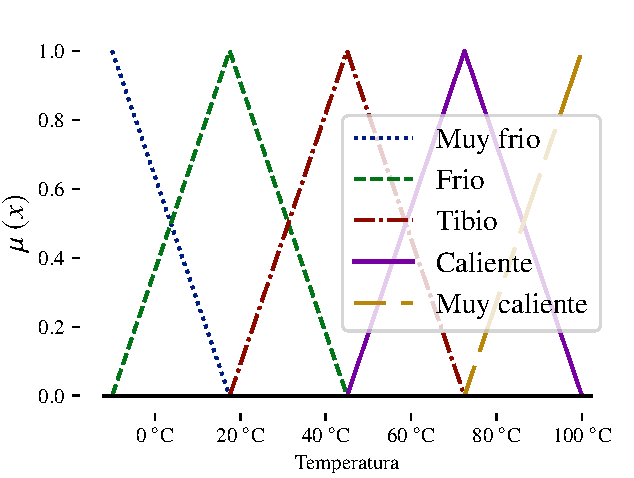
\includegraphics[width=0.6\linewidth]{imagenes/FuzzySet.pdf}
	\end{figure}
	\vspace{-20pt}
	\begin{itemize}
		\Large
		\item Python
	\end{itemize}

\end{frame}

\begin{frame}
	\frametitle{ESTRUCTURA DEL CÓDIGO: UML}
	\vspace{20pt}
	\begin{figure}
		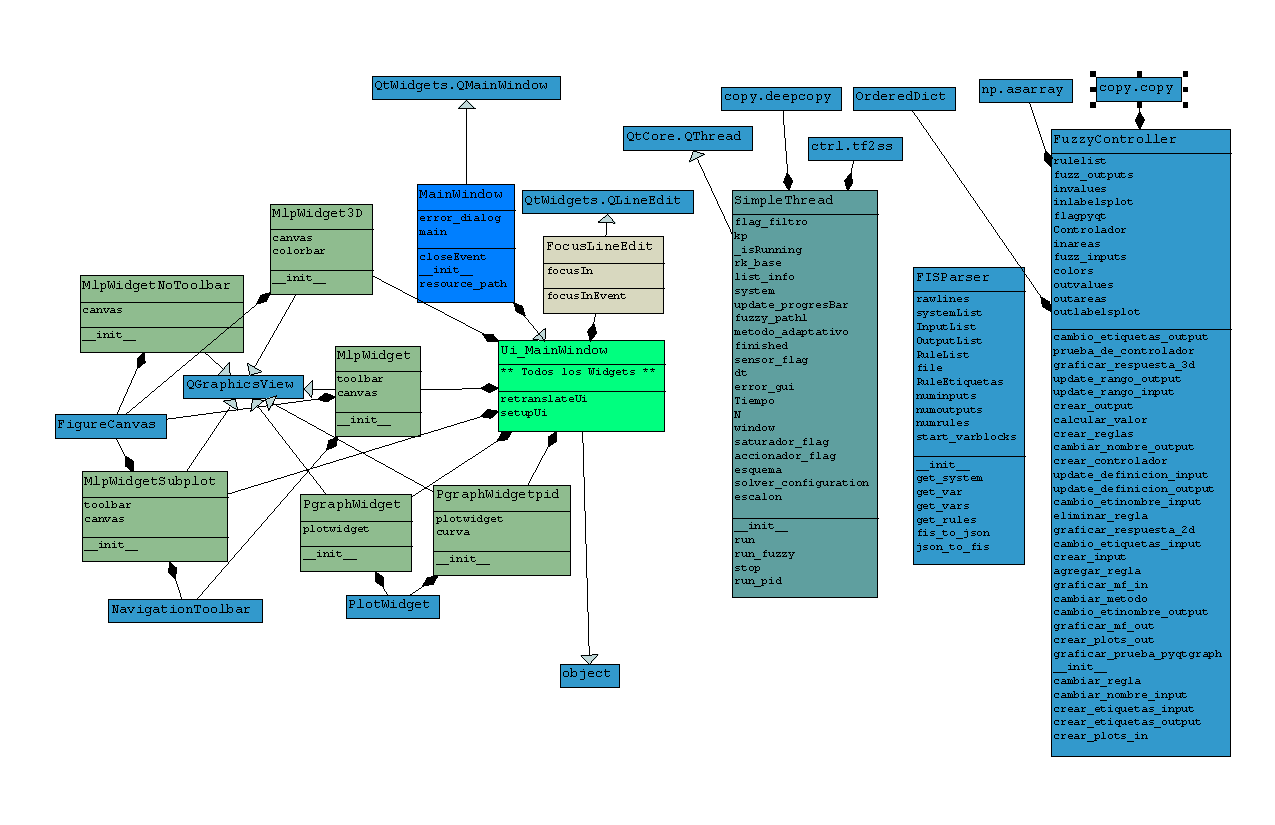
\includegraphics[width=\linewidth]{imagenes/UMLsinHandlers.pdf}
	\end{figure}
\end{frame}

\begin{frame}
	\frametitle{ESTRUCTURA DEL CÓDIGO: ESQUEMA}
	\vspace{20pt}
	\begin{figure}
		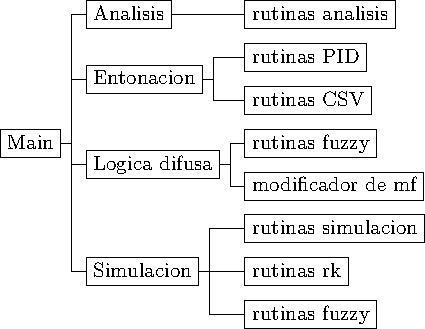
\includegraphics[width=0.9\linewidth]{imagenes/estructuraMain.pdf}
	\end{figure}
\end{frame}

\begin{frame}
	\frametitle{COMPARACIÓN}
	\framesubtitle{ANÁLISIS}
	% \vspace{20pt}
	\rowcolors{1}{UniBlue!33}{UniBlue!7}
	{\centering
	\begin{table}[t]
		\centering 
		\hspace*{-0.6cm}
		\begin{threeparttable}
			% \setlength{\tabcolsep}{6pt}			% Separacion de columnas
			\setlength{\arraycolsep}{1pt}
			\scriptsize
			\renewcommand{\arraystretch}{3}
			\caption[Sistemas para la comparación de análisis de sistemas de control]{Sistemas para la comparación de análisis de sistemas de control}
			\begin{tabular*}{\textwidth}{c @{\extracolsep{\fill}}c}
					 {\normalsize Continuo} & {\normalsize Discreto} \\\renewcommand{\arraystretch}{3}
			$\dfrac{1}{s^2 + s + 1} $ & $\dfrac{0.004833 z+0.004675}{z^2 - 1.895 z + 0.9048} $  \\[5pt]
			\begin{tabular}[x]{cc} \setlength\arraycolsep{2pt} \renewcommand{\arraystretch}{1} $\begingroup \setlength\arraycolsep{2pt} A=\begin{colorbmatrix} -0.5 & -3 & -0.2 \\
				1 & 0 & 0 \\
				0 & 1 & 0 
			\end{colorbmatrix} \endgroup $ &  \renewcommand{\arraystretch}{1}
			$B=\begin{colorbmatrix} 1 \\ 0 \\ 0 \end{colorbmatrix}$ \\ \renewcommand{\arraystretch}{1}
			$C=\begin{colorbmatrix} 1 & 2 & 0.5 \end{colorbmatrix}$ & \renewcommand{\arraystretch}{1}
			$D=\begin{colorbmatrix} 0 \end{colorbmatrix}$ \end{tabular} & \begin{tabular}[x]{cc} \renewcommand{\arraystretch}{1} $A=\begin{colorbmatrix} 851.5 & -559.2 & -37.03 \\
				185.2 & 944.1 & -3.703 \\
				18.52 & 194.4 & 999.6 
			\end{colorbmatrix}_{10^{-3}} $ &  \renewcommand{\arraystretch}{1}
			$B=\begin{colorbmatrix} 185.2 \\ 18.52 \\ 1.852 \end{colorbmatrix}_{10^{-3}}$ \\ \renewcommand{\arraystretch}{1}
			$C=\begin{colorbmatrix} 1.116 & 1.713 & 0.4777 \end{colorbmatrix}$ & \renewcommand{\arraystretch}{1}
			$D=\begin{colorbmatrix} 0.1116 \end{colorbmatrix}$ \end{tabular} \\[15pt] 
			$\dfrac{s + 2}{s^2 + 0.5s + 3}e^{-1.5s} $ & $z^{-30}\left(\dfrac{0.02561 z^2 + 0.003084  z - 0.02375}{z^2 - 1.968 z + 0.9753}\right)$\\[8pt]
			\end{tabular*}
			\label{tab:AnalisisSistemas}
		\end{threeparttable}
	\end{table}}
\end{frame}

\begin{frame}
	\frametitle{COMPARACIÓN}
	\framesubtitle{ANÁLISIS}
	\vspace{21pt}
	\small
	\begin{block}{Funciones de análisis}
		\footnotesize
		\begin{multicols}{2}
		\begin{itemize}
			\item Respuesta al escalón
			\item Respuesta al impulso
			\item Bode
			\item Nyquist
			\item Lugar de las raíces 
			\item Diagrama de Nichols
		\end{itemize}
	\end{multicols}
	\end{block}

	\begin{block}{Metricas empleadas}
		\footnotesize
		\begin{multicols}{2}
		\begin{itemize}
			\item Diferencia absoluta
			\item Diferencia porcentual
			\item Diferencia de área
			\item Raíz del error cuadrático medio (RECM)
			\item Distancia de energía
		\end{itemize}
	\end{multicols}
	\end{block}

	\vspace{-5pt}
	\rowcolors{1}{UniBlue!33}{UniBlue!7}
	\begin{table}
		\begin{tabular}{rcc}
										& Continuo 			& Discreto 			\\
		Diferencia porcentual promedio	& \num{5.065E-01}	& \num{3.333E-01}	\\
		RECM promedio					& \num{1.644E-02}	& \num{1.307E-02} 	\\
		\end{tabular}
	\end{table}
\end{frame}

\begin{frame}
	\frametitle{COMPARACIÓN}
	\framesubtitle{ANÁLISIS}
	\vspace{25pt}
	\begin{figure}
		\begin{subfigure}[t]{0.49\linewidth}
			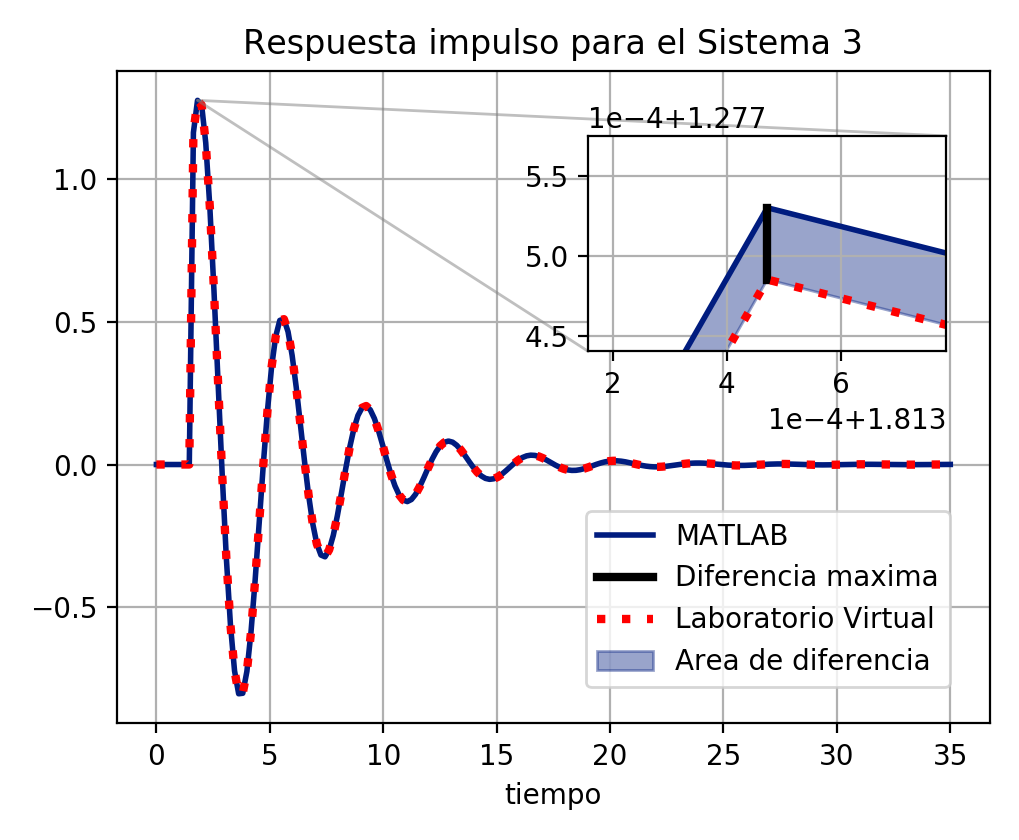
\includegraphics[width=\linewidth]{imagenes/Set3Imp.png}
			\caption{}
		\end{subfigure}
		\hfill
		\begin{subfigure}[t]{0.49\linewidth}
			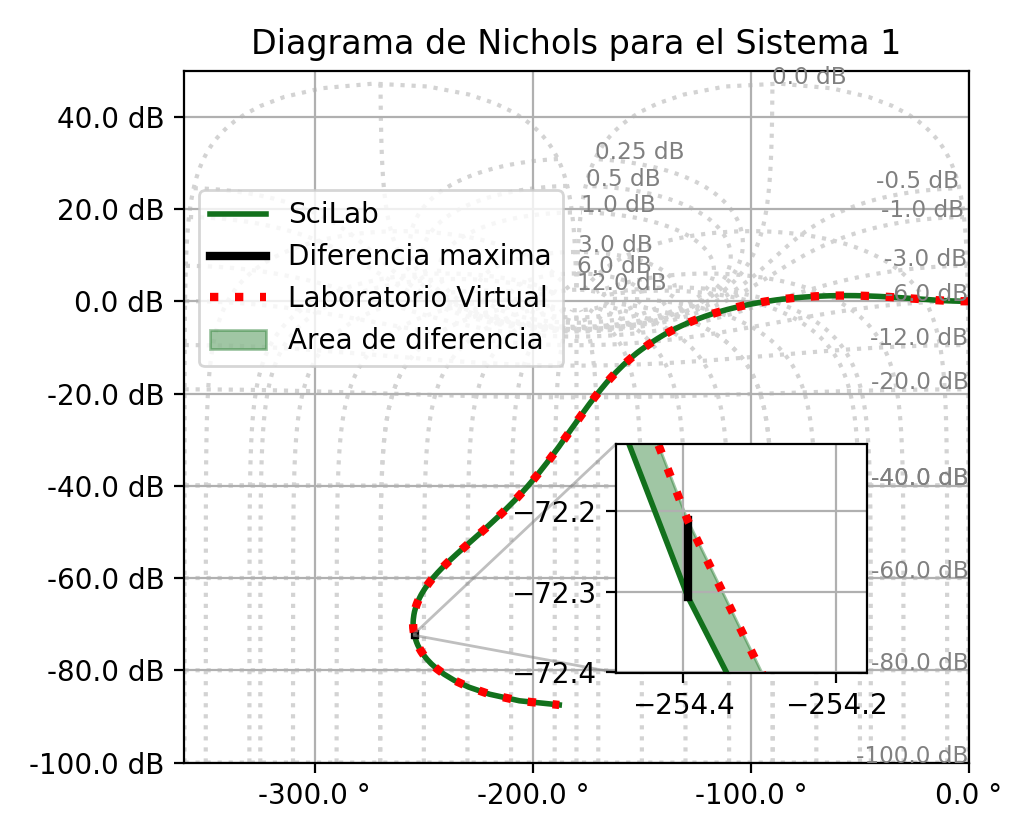
\includegraphics[width=\linewidth]{imagenes/ScSet1DNichols.png}
			\caption{}
		\end{subfigure}
		\caption{Gráficas de comparación para la función de análisis. (a) Respuesta impulso para el sistema 3 en tiempo continuo, (b) Diagrama de Nichols para el sistema 1 en tiempo discreto.}
	\end{figure}

\end{frame}

\begin{frame}
	\frametitle{COMPARACIÓN}
	\framesubtitle{CONTROLADORES DIFUSOS}
	\vspace{25pt}
	\rowcolors{1}{UniBlue!33}{UniBlue!7}
	\begin{table}
		\begin{tabular}{rcc}
						& MATLAB 			& SciLab 			\\
		Controlador 1	& \num{1.10E-01}\%	& \num{1.10E-01}\%	\\
		Controlador 2	& -					& \num{0.00E-00}\%	\\
		\end{tabular}
	\end{table}

	\begin{figure}[htb]
		\centering
		\begin{subfigure}[t]{0.32\textwidth}
			\centering
			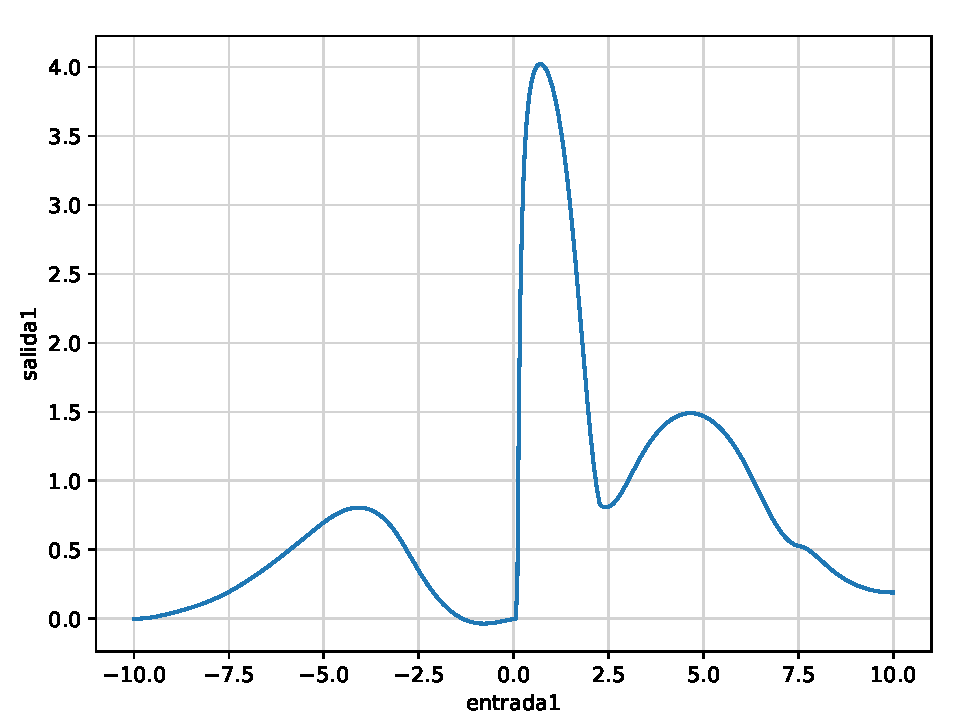
\includegraphics[width=\textwidth]{imagenes/LVTomoC1.pdf}
			\caption{}
		\end{subfigure}
		\hfill
		\begin{subfigure}[t]{0.32\textwidth}
			\centering
			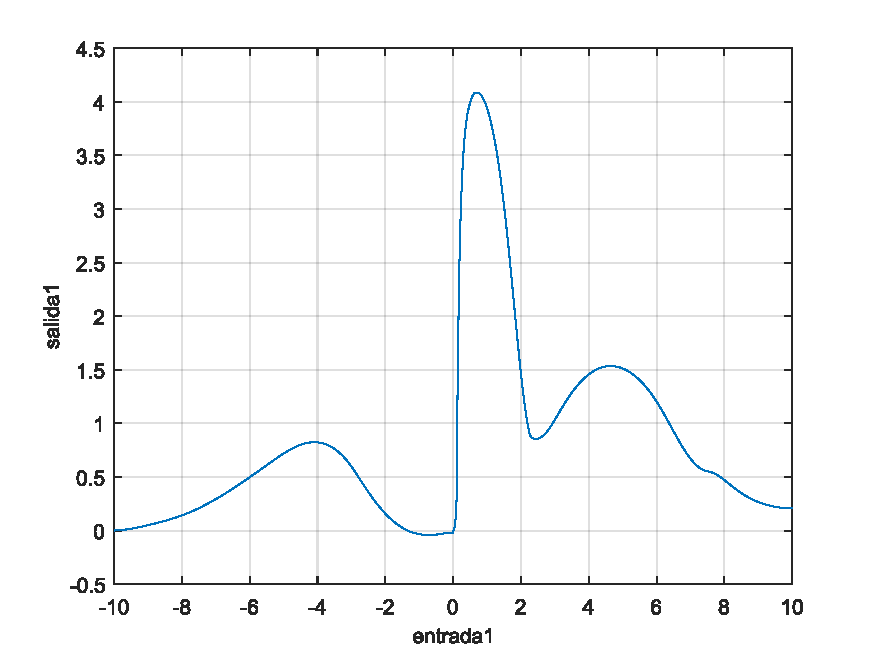
\includegraphics[width=\textwidth]{imagenes/MATLABTomoC1.pdf}
			\caption{}
		\end{subfigure}
		\hfill
		\begin{subfigure}[t]{0.32\textwidth}
			\centering
			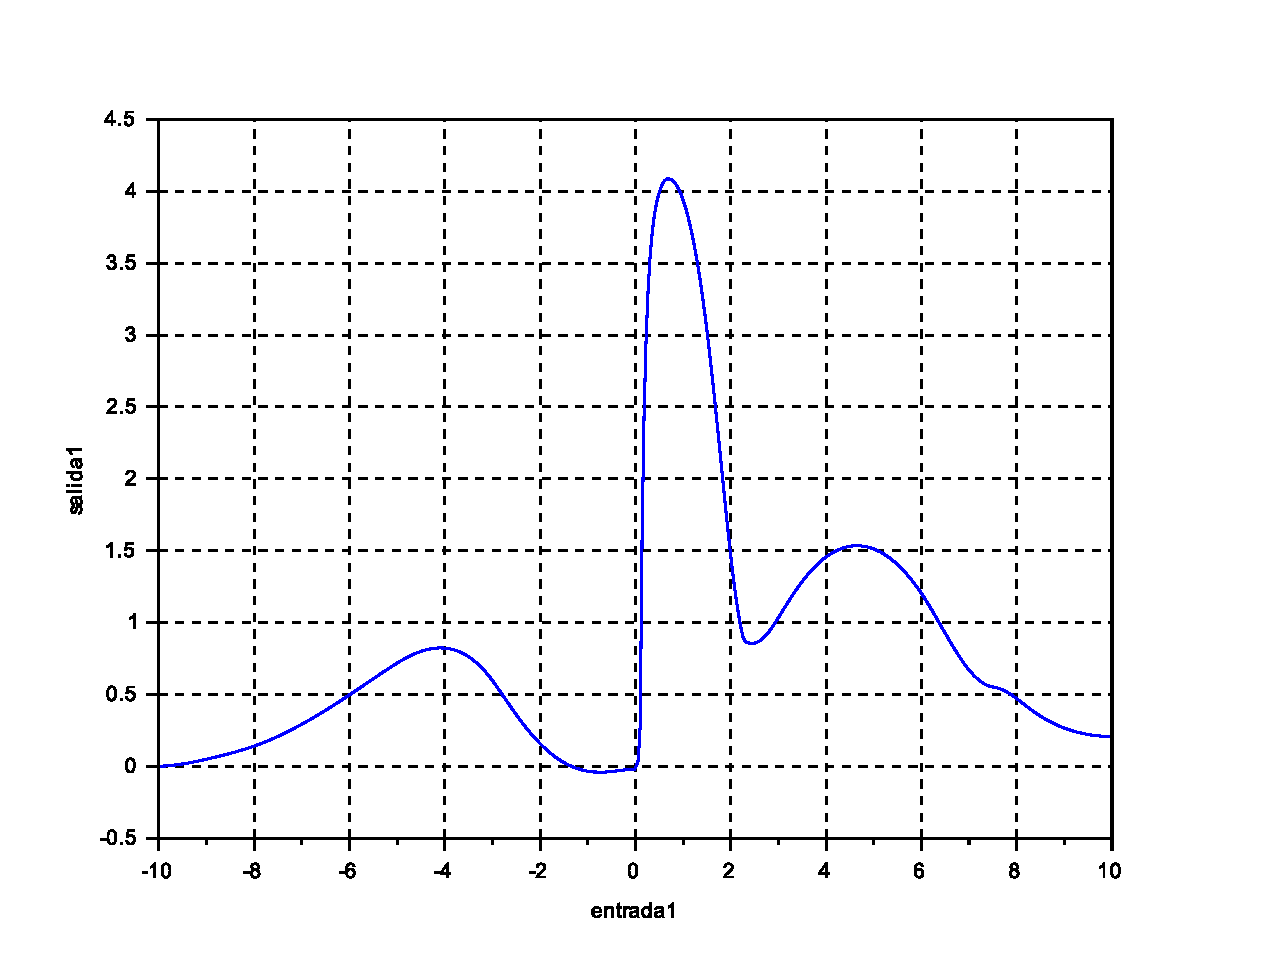
\includegraphics[width=\textwidth]{imagenes/SciLabTomoC1.pdf}
			\caption{}
		\end{subfigure}
		\caption{Respuesta del controlador difuso 1. (a) Laboratorio Virtual, (b) MATLAB, (c) SciLab.}
	\end{figure}

\end{frame}

\begin{frame}
	\frametitle{COMPARACIÓN}
	\framesubtitle{SIMULACIÓN}
	\vspace{20pt}
	\begin{block}{Condiciones}
		\begin{itemize}
			\item Tiempo continuo
			\begin{itemize}
				\item[--] Distintos solvers
				\item[--] Tolerancia absoluta y relativa distinta según el solver
				\item[--] Con y sin filtro derivativo (para el Laboratorio Virtual)
			\end{itemize}
			\item Tiempo discreto
			\begin{itemize}
				\item[--] Condiciones iguales para las tres (3) herramientas
				\item[--] Periodos de muestreo y métodos de discretización variados
				\item[--] Una sola prueba por tipo de controlador
			\end{itemize}
		\end{itemize}
	\end{block}

	\begin{alertblock}{Nota!}
		Todos los controladores diseñados son inadecuados para el control de procesos.
	\end{alertblock}

\end{frame}

\begin{frame}
	\frametitle{COMPARACIÓN}
	\framesubtitle{SIMULACIÓN}
	\vspace{21pt}
	\begin{figure}[htb]
		\centering
		\begin{subfigure}[t]{0.49\textwidth}
			\centering
			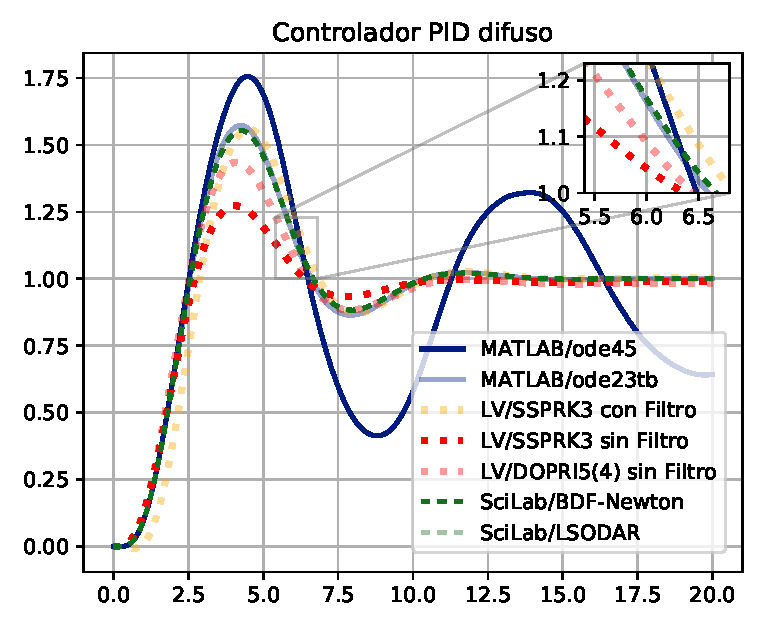
\includegraphics[width=\textwidth]{imagenes/PIDcf1.pdf}
			\caption{}
		\end{subfigure}
		\hfill
		\begin{subfigure}[t]{0.49\textwidth}
			\centering
			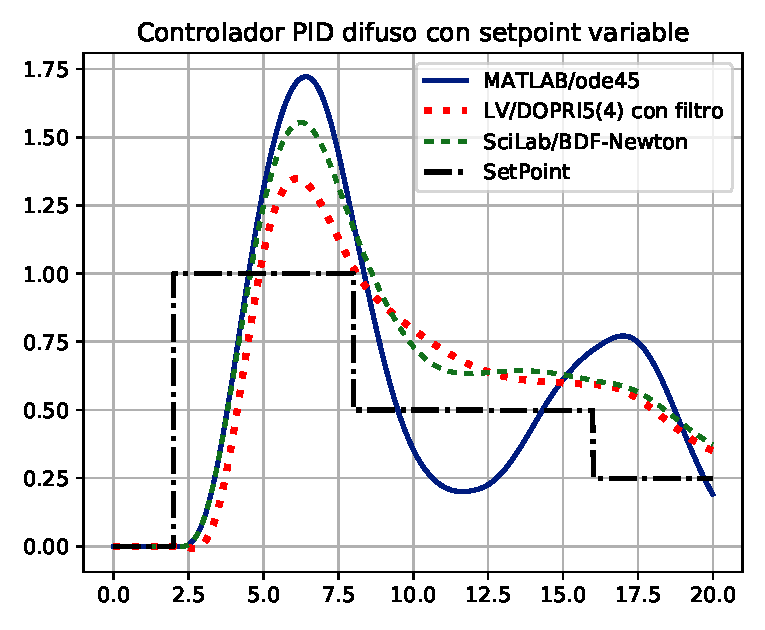
\includegraphics[width=\textwidth]{imagenes/PIDcf2.pdf}
			\caption{}
		\end{subfigure}
		\caption{Simulación de esquemas difusos. (a) PID difuso con setpoint constante, (b) PID difuso con setpoint variable. Ambos en tiempo continuo}
	\end{figure}

\end{frame}

\begin{frame}
	\frametitle{COMPARACIÓN}
	\framesubtitle{SIMULACIÓN}
	\vspace{23pt}
	\begin{figure}[htb]
		\centering
		\begin{subfigure}[t]{0.49\textwidth}
			\centering
			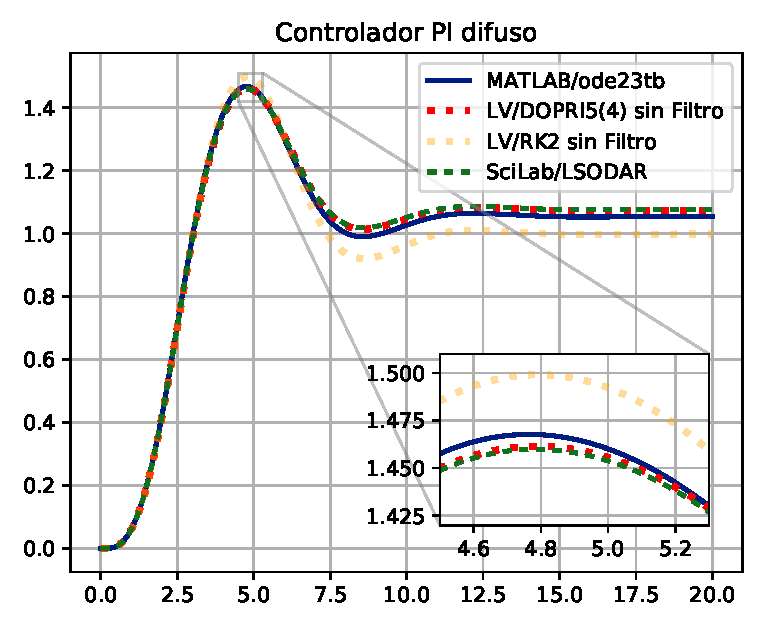
\includegraphics[width=\textwidth]{imagenes/PIcf1.pdf}
			\caption{}
		\end{subfigure}
		\hfill
		\begin{subfigure}[t]{0.49\textwidth}
			\centering
			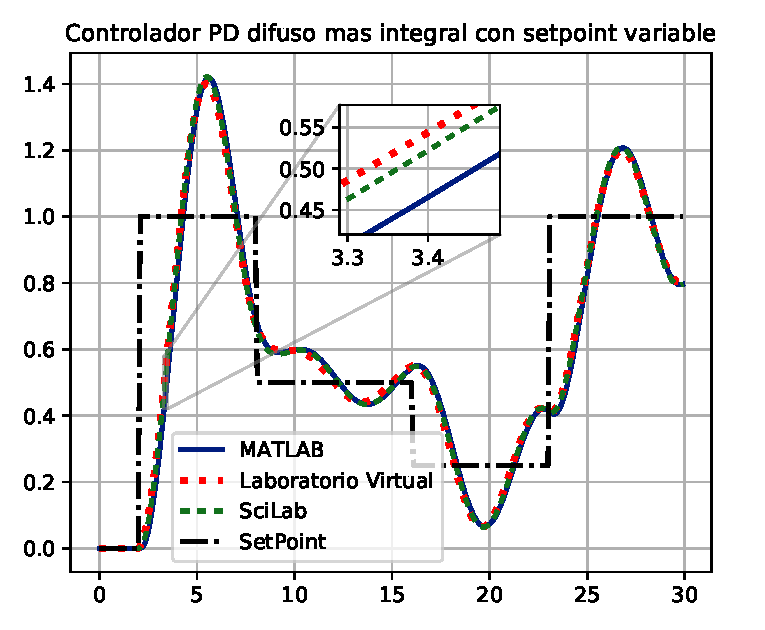
\includegraphics[width=\textwidth]{imagenes/PDmasId.pdf}
			\caption{}
		\end{subfigure}
		\caption{Simulación de esquemas difusos. (a) PI difuso con setpoint constante en tiempo continuo, (b) PD difuso más Integral con setpoint variable en tiempo discreto.}
	\end{figure}

\end{frame}

\begin{frame}
	\frametitle{CONCLUSIONES}
	\small
	\vspace{20pt}
	\begin{enumerate}
        \item Todas las funciones implementadas presentaron, en su mayoría, resultados cercanos dentro de una tolerancia a las herramientas alternas que se consideraron, logrando así demostrar que es posible realizar un Laboratorio Virtual de sistemas de control utilizando software libre.
        
        \item El Laboratorio Virtual, aunque potente, se encuentra aún limitado en funciones respecto a otras herramientas como MATLAB y SciLab, esto es esperable ante el alcance planteado en este trabajo y se considera que herramientas como Simulink y Xcos para la simulación de sistemas de control son aún superiores.
		
		\item La librería Scikit-Fuzzy carece de la optimización necesaria para poder realizar simulaciones en lotes, i.e., posee tiempos de ejecución altos para procesar una simulación con múltiples muestras de un tiempo total dado. Lo anterior se entiende dado que Scikit-Fuzzy está pensada para diseñar controladores difusos que serán implementados en microcontroladores, no obstante, el Laboratorio Virtual logra mejorar los tiempos de ejecución de SciLab en algunas situaciones.
    \end{enumerate}

\end{frame}

\begin{frame}
	\frametitle{CONCLUSIONES}
	\small
	\vspace{15pt}
	\begin{enumerate}
		\setcounter{enumi}{3}
		\setlength\itemsep{1em}      
        \item El Laboratorio Virtual logra ofrecer las herramientas necesarias para realizar análisis, diseño y simulación de controladores clásicos y difusos de forma simple y rápida sin tener que escribir una línea de código gracias a la interfaz de usuario implementada.
        
        \item El Laboratorio Virtual posee un gran potencial como herramienta para ingenieros en el área de los sistemas de control y posee un diseño tal que permite seguir siendo desarrollada en esta área, adicionalmente, Python ofrece una gran variedad de librerías externas que pueden emplearse para expandir el Laboratorio Virtual en otros ámbitos sin la necesidad de tocar las funciones ya implementadas.
    \end{enumerate}

\end{frame}

\begin{frame}
	\frametitle{RECOMENDACIONES}
	\small
	\vspace{20pt}
	\begin{enumerate}   
		\item Re implementar el sistema de inferencia difuso de Scikit-Fuzzy asegurándose de no modificar los sistemas de diseño de controladores, lo anterior permitiría poder procesar de forma más rápida grandes cantidades de datos con la finalidad de acortar los tiempos de simulación en la función de simulación de sistemas de control sin que, a su vez, se tenga que volver a codificar el archivo ``Handler'' correspondiente.
		
		\item Implementar la posibilidad de diseñar y simular los sistemas de inferencia Takagi-Sugeno-Khan y Tsukamoto, los cuales son más acordes y utilizados en el área de los sistemas de control, adicionalmente, se puede incluir el controlador Larsen.
		
		\item Añadir una nueva función que incorpore un sistema SCADA con la finalidad de poner a prueba los controladores diseñados de forma experimental, para ello se puede utilizar las distintas librerías existentes que incorporan múltiples protocolos de comunicación, i.g., modBuss.
		
	\end{enumerate}

\end{frame}

\begin{frame}
	\frametitle{RECOMENDACIONES}
	\vspace{15pt}
	\small
	\begin{enumerate}
		\setcounter{enumi}{3}
		\setlength\itemsep{1em} 
		\item Implementar algoritmos de resolución de sistema de ecuaciones diferenciales para problemas stiff como BDF y LSODAR que ofrecen mejores precisiones que las obtenidas con los métodos explícitos y embebidos.
		
		\item Implementar una consola que permita codificar Python dentro del Laboratorio Virtual y que se pueda distribuir utilizando un único archivo ejecutable, de este modo se obtendría una herramienta más completa y potente que permitiría realizar cálculo numérico y simbólico, graficacion y codificación general.
	\end{enumerate}
	

\end{frame}
\end{document}